\chapter{Development Process \& Contributing to MATSim}
\label{ch:developmentprocess}
% ##################################################################################################################

\hfill \textbf{Authors:} Andreas Horni, Marcel Rieser, Kai Nagel

\begin{center} 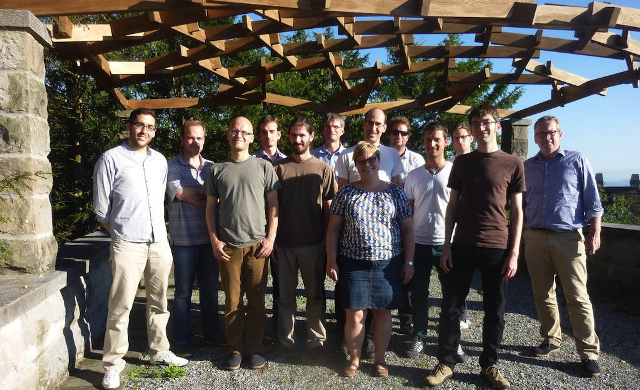
\includegraphics[width=0.5\textwidth, angle=0]{extending/figures/ConceptualMeetingVillaHatt.png} \end{center}

% ##################################################################################################################
This chapter describes how new functionality enters MATSim. It describes the MATSim team and community, the different roles existing in the MATSim project, development drivers and processes, and tools used for integration. The goal is to give you an overview on the development process such that you quickly find access to the MATSim community and such that you are able to efficiently contribute to MATSim according to one role or another, if you commendably like to.

% ##################################################################################################################
\section{MATSim Team and MATSim Community}
The MATSim team, the heart of the MATSim community, are three research groups and a spin-off company, namely 
\begin{itemize}
\item the Transport Systems Planning and Transport Telematics group at the Institute for Land and Sea Transport Systems, Technische Universität Berlin, led by Prof.\ Dr.\ Kai Nagel,
\item the Transport Planning group at the Institute for Transport Planning and Systems (IVT), Swiss Federal Institute of Technology Zürich, led by Prof.\ Dr.\ Kay W.\ Axhausen, 
\item the recently founded Mobility and Transportation Planning group at the Future Cities Laboratory, based in Singapure and lead by Prof.\ Dr.\ Kay W.\ Axhausen, and 
\item senozon AG, based at Zürich with a subsidiary in Germany, founded by former PhD and research students. 
\end{itemize}

As common in research the universities groups' composition changes frequently. Over the last decade more than 50 people build the MATSim core as listed earlier.

Besides the MATSim team, there is a community composed of closely connected research groups (such as Stockholm, Pretoria, Poznan, Jülich and Toronto) and more loosely connected external users coming together at the annual MATSim user meeting.   

MATSim is an open-source program provided by the GNU General Public License version 2.0 (GPLv2), thus, you are also very welcome to contribute to the code base as described in Section~\ref{sec:yourcontribution}. Further contributors are mentored in the beginning \citep[][]{MATSIM-T-BecomingAContributor_Webpage_2014} to become familiar with the project and the coding conventions \citep[][]{MATSIM-T-CodingGuide_Webpage_2014}.

Picture \ref{fig:team} shows a snapshot of the participants of the first conceptual meeting representing a good mix of core group members but also associated researchers.
%
% ------------
\createfigure%
{Participants of the first MATSim conceptual meeting at Villa Hatt in Zürich in 2012}%
{Participants of the first MATSim conceptual meeting at Villa Hatt in Zürich in 2012}%
{\label{fig:team}}%
{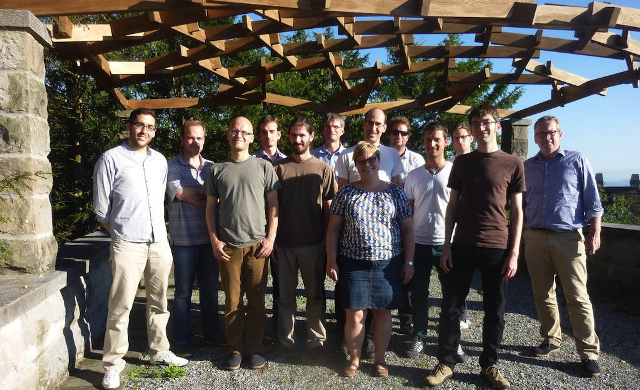
\includegraphics[width=0.99\textwidth, angle=0]{extending/figures/ConceptualMeetingVillaHatt.png}}%
{}
% ------------

% ##################################################################################################################
\section{Roles in the MATSim community}
\label{sec:roles}
There are the following roles in the MATSim community.
%
\begin{compactitem}
\item The \textbf{MATSim user} uses the official releases or nightly builds and runs MATSim with the config file. Part I of the book is dedicated to the MATSim user. On the web page he or she finds relevant information in the \emph{user's guide} and in the user's mailing list \lstinline|matsim-users@lists.sourceforge.net|.
\item The \textbf{MATSim API-user} extends MATSim by programming against the MATSim-API. He or she finds his or her information in Part II of the book, in particular in Chapter~\ref{ch:extensionpoints}, on the web page in the \emph{API-user's guide} and in the mailing list \lstinline|matsim-devel@lists.sourceforge.net|.
\item The \textbf{MATSim developer} also programs against the MATSim-API, but additionally he or she is part of the MATSim code base by having his or her own playground or contribution being part of the refactorings. 
%\ah{contribs auch, oder?} \kai{ja}. 
The developer finds information in Part II of this book, on the web page in the \emph{developer's guide} and in the mailing list \lstinline|matsim-devel@lists.sourceforge.net| 
\item There are relatively few \textbf{MATSim core developers} stemming from the MATSim team. These role is an extension of the MATSim developer and these guys make necessary modifications of the core code (\lstinline|package org.matsim.core.*| see next section), usually after having discussed them in the MATSim committee or at a developer meeting (see below). Part III of this book might be particularly interesting for them.
\end{compactitem}
%
% ##################################################################################################################
\section{Drivers and Organization of Development}
Main drivers of the MATSim development are the projects and dissertations accomplished by the MATSim team. New features are developed as an answer to requirements of these dissertations and projects, where projects range from purely scientific ones (often sponsored by SNF) to projects for the administration, to projects where science and industry contribute equally (usually CTI-projects) and to purely industrial projects, which are managed by senozon AG in the majority of cases. A significant amount of innovation is also introduced by the collaboration with external researchers.

Systematic code integration is mainly performed by the Berlin group and by senozon AG. This includes continuous code review and integration upon request of the community, but also comprehensive code refactorings to clean degenerated code. Refactorings are documented in the MATSim issue tracker.

The development process is supported by a standing MATSim committee discussing conceptual issues on a regular basis. Another element bringing in innovation but also organization are the annual meetings. Right from the beginnings, there has been a MATSim developer meeting focused on coding issues. Later, a user meeting giving insights into accomplished work by the community has been invented. Finally, a conceptual meeting has been added strictly dedicated to issues that go beyond pure software engineering. The developer and the conceptual meeting have shown to establish an effective road map, which has guided the development for the remainder of the year. 

The internal development is organized by regular group meetings, in Zürich for example by the ``MATSim group meeting'' and in Berlin by the ``jour fix''. 

Due to the heterogeneous character of the community and its individual research groups, with every member being engaged in his individual dissertation work, organizing the development in an agile and somewhat ad hoc manner has been regarded beneficial over adopting an established and strict software project management method.

% ##################################################################################################################
\section{Code Base, Development Tools and Techniques}
The main part of the MATSim code base is the MATSim project \lstinline|org.matsim.*|. Additionally, there is not directly related to the core functionality of MATSim, which is agent-behavior and transport simulation, is available in the code base as MATSim contributions (\lstinline|package org.matsim.contrib.*|). Such modules are usually provided by MATSim API-users or developers. Finally, there are the developers' playgrounds.

Since the huge refactoring greatly improving the code base structure and establishing, the MATSim project code is divided into the \emph{core} \lstinline|org.matsim| and \emph{api} packages \lstinline|org.matsim.api| and remaining packages. This refactoring was undertaken by the Berlin group starting at the end of 2007 and ended in the beginning of 2009 before the first user meeting \ah{stimmt das so?}.

In the early days of MATSim, the code was programmed in \emph{C++}. Later, however, the code was migrated to \emph{Java}. Performance of \emph{Java} and \emph{C++} had converged to a reasonable extent, such that the much higher developer friendliness of Java could be exploited. A fast access to the program is essential for MATSim as many API-users have their background in fields such as transport planning or social sciences and not in computer science. 

Up to 2007, when MATSim was brought to \emph{Sourceforge}, MATSim was provided by a download website and svn repository hosted on a VSP server.

MATSim development makes use of a whole bunch of tools greatly leading to better software quality. Summarized and accessible from the MATSim website---with private access---a change log, an issue tracker, the \emph{javadoc}, static code analyses performed by \emph{FindBugs} and \emph{PMD}, test code coverage analysis, copy paste analysis, code metrics, \emph{maven} dependencies, the complete code linked by \emph{Xref}, and the information about the nightly test results are provided. These nightly test results are generated by the MATSim build server based on \emph{Jenkins}. Furthermore, there is a MATSim benchmark available \url{http://www.matsim.org/docs/devguide/optimization}.

Most MATSim developers use \emph{Eclipse} as an integrated development environment (IDE). The MATSim documentation is tailored to this IDE. Team development is based on \emph{Apache Subversion SVN}. External libraries dependencies are managed by \emph{Maven}. 

MATSim development furthermore greatly benefits from the possibility to run large-scale scenarios. Therefore, several servers with up to 512GB RAM and 40 CPU cores are available.  

% ##################################################################################################################
\section{Documentation, Dissemination and Support}
The main documentation can be found on the MATSim web page \citep[][]{MATSIM-T-Docu_Webpage_2014}, where information is distinctly provided in the three guides mentioned above. Additionally, a handful of tutorials is available, with the ``Quickstart''-tutorial to get fast access to MATSim and the ``Learning MATSim in 8 Lessons''-tutorial, which is used for the user's meetings and hands-on tutorials in Berlin, Zürich and occasionally elsewhere, also listed on that page. 

Code documentation in form of \emph{Javadoc} can be found at \citet[][]{MATSIM-T-Javadoc_Webpage_2014}, as cross references view (Xref) \url{http://matsim.org/xref} and as doxygen documentation \url{http://matsim.org/doxygen}. %\kai{gerne auch xref und doxygen URLs: \url{http://matsim.org/xref} and \url{http://matsim.org/doxygen}.}

For fast application of MATSim some small-scale example scenarios are provided in the code base (\lstinline|folder: src/test/resources/test/scenarios/|), where recently an extended version of the well-known benchmark scenario for the City of Sioux Falls has been added \citep[][]{ChakirovFourie_TechRep_FCL_2014}.

Further information is disseminated at the afore-described annual user meetings and MATSim mailing lists. Usually, also support is provided by the MATSim team via these mailing lists. Particularly active in support are the Berlin group and senozon AG. A theoretical overview of all the components in MATSim is given by the numerous papers published in international journals and presented at worldwide conferences; an overview can be found at \citep[][]{MATSIM-T-Publications_Webpage_2014} and in this book's part II.

Apparently, the information on MATSim is quite extensive, however, getting a complete picture as a new MATSim user requires a substantial literature search effort. Reduction of this hassle is the goal of the book at hand.

% ##################################################################################################################
\section{Your Contribution to MATSim}
\label{sec:yourcontribution}
The technical details, i.e., the MATSim extensions points where to hook with MATSim are detailed in the next Chapter. Here, the different ways of contributing to MATSim according to the roles presented in Section~\ref{sec:roles} are introduced.

As a user or API-user you are warmly welcome to make an important impact by reporting your achievements, needs and problems with, or bugs of, the software via the users mailing list or at the annual MATSim user meeting. 

If you would like to directly contribute to the code base of MATSim you are welcome to become a MATSim developer with your own playground or contribution.

If you are the type of guy that likes to change the core system, you can, although it is a long way, become a MATSim core developer. Core developers are usually picked from the MATSim team. Prerequisites are a strong computer scientist background, several years of experience with MATSim and a deep understanding of large software projects.

% ##################################################################################################################
%\section{Discussion and TODOs}
%\label{sec:development_process}
%Will be commented, when chapter is finished. Make final results traceable.
%
%% --------------
%\kai{Ich würde gerne ``Development process'' und ``Contributing to MATSim'' auftrennen.  Ersteres beschreibt Dinge wie core development, regression tests, etc.  Aber ``contributing to MATSim'' sollte sich auf die extension points konzentrieren.  Vielleicht zusammen mit dem vorhergehenden Kapitel.}
%
%\kai{Bin mir allerdings beim zweiten Nachdenken nicht mehr sicher, ob das so kategorisch sein muss.  Wir sollten erstmal versuchen, ``contributing to matsim'' als logische Folge des development process zu schreiben.  Dann sind ``minimally invasive contributions'' ja gerade solche, welche die extension points verwenden.}
%
%% --------------
%\ah{Vieles noch etwas zu implizit dargestellt! -> Aufzählungen einfügen. Playgrounds! Testing! Verantwortlichkeiten!}
%
%% --------------
%\ah{Classes und Methods stabil seit Langem: 
%auf was deutet das hin? Zu wenig Innovation oder Clean-Code? Steckt zuviel in den Playgrounds, Contribs oder ist das genau richtig?
%Wurde Kernfunktionalität eingefügt und dafür weniger Zentrales (wie Evacuation) nach und nach in Contrib verschoben?}
%
%\ah{Der Drop Ende 2007, war das schon Core, API Umstruktutierung oder war das die Entfernung von G. package?}
%\kai{Entfernung von Gunnar's package.}
%
%\createfigure%
%{Code development since 2005}%
%{Code development since 2005}%
%{\label{fig:codedev}}%
%{%
  %\createsubfigure%
  %{...}%
  %{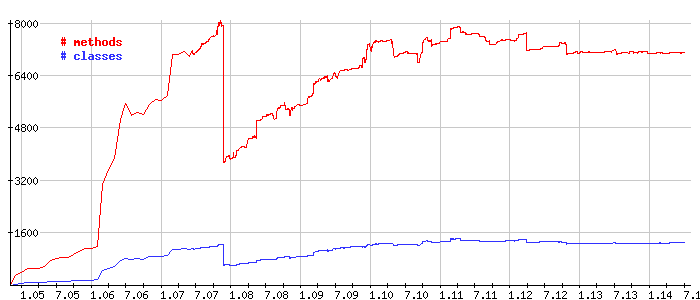
\includegraphics[width=0.95\textwidth,angle=0]{extending/figures/nof_classes.png}}%
  %{\label{fig:codedev0}}%
  %{}%
  %\createsubfigure%
  %{...}%
	%{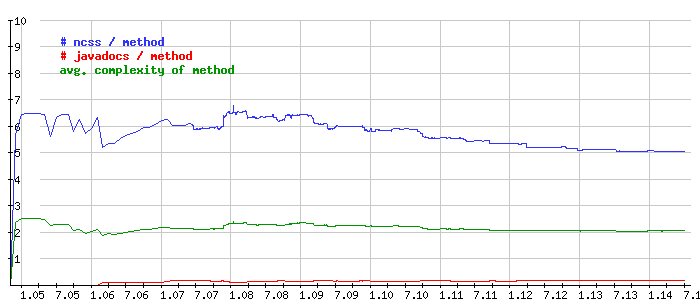
\includegraphics[width=0.95\textwidth,angle=0]{extending/figures/avg_method.png}}%
  %{\label{fig:codedev1}}%
  %{}%
%}%
%{}
%
%
%\ah{noch weiter eingehen auf Code Struktur? Resources, XML, ect.???}
%\ah{approx. number of playgrounds}
%\ah{approx number of code lines /classes at the different locations (core, playgrounds, contributions etc.}

% ##################################################################################################################
